% id: 150-11
% book: 100발100중 3-1 기말 · 01 3-1 기말(이차방정식·이차함수·부록)
% section: 파이널 모의고사 2회
% figure: crop:fig-150-11.png
% answer: ③
% answer_source: 답지(빠른정답)
% variant_level: 0 (원본 전사)
% 이 파일은 build.mjs 가 items.json 에서 만든다. 고칠 때는 items.json 을 고친다.
\smash{\raisebox{1.5mm}{\dmkichul{100발100중 3-1 기말 150쪽 11번}}}
\noindent\begin{minipage}[t]{0.58\linewidth}\vspace{0pt}\raggedright 그림과 같이 $\seg{AD}=15\mkern3mu \mathrm{cm}$, $\seg{DC}=10\mkern3mu \mathrm{cm}$인 직사각형 $\pt{ABCD}$에서 점~$\pt{P}$는 점~$\pt{A}$를 출발하여 점~$\pt{B}$까지 초속 $1\mkern3mu \mathrm{cm}$의 속력으로, 점~$\pt{Q}$는 점~$\pt{B}$를 출발하여 점~$\pt{C}$까지 초속 $3\mkern3mu \mathrm{cm}$의 속력으로 움직이고 있다. 이때 $\triangle\pt{PBQ}$의 넓이가 $36\mkern3mu \mathrm{cm}^2$가 되는 것은 두 점 $\pt{P}$, $\pt{Q}$가 동시에 출발한 지 몇 초 후인가? \mbox{[4점]}\end{minipage}\hfill\begin{minipage}[t]{0.4\linewidth}\vspace{0pt}\centering 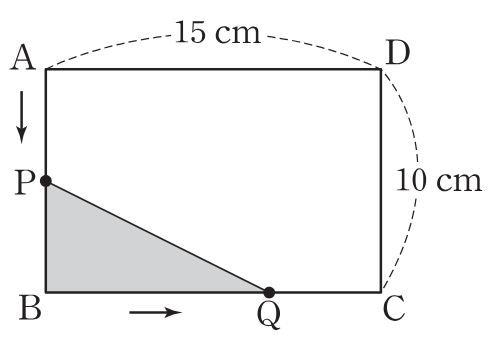
\includegraphics[width=117.9pt]{figures/fig-150-11.png}\end{minipage}\par
\begin{choices32}{$2$초 후}{$3$초 후}{$4$초 후}{$5$초 후}{$6$초 후}\end{choices32}
